\chapter{Shortest Paths}
\label{ch:shortest-paths}

\newcommand{\visited}{X}
\newcommand{\unvisited}{T}
\newcommand{\ev}{\sml{eVal}}
\newcommand{\dist}{\delta}
\newcommand{\sssp}{\probName{SSSP}}
\newcommand{\ssspp}{\probName{SSSP$^+$}}
\newcommand{\ssspd}{\probName{SSSP$_{\dist}$}}
\newcommand{\sssppd}{\probName{SSSP$^+_{\dist}$}}

\begin{todo}
 weight ==> length, this is more consistent with "shortest"
 weight would make "lightest" to be a better word.
\end{todo}

\begin{todo}
Are we talking about paths or simple paths? it seems like paths,
allowing for reps.
\end{todo}

Given a graph where edges are labeled with weights (or distances) and
a source vertex, what is the shortest path between the source and some
other vertex?  Problems requiring us to answer such queries are
broadly known as \defn{shortest-paths problems}. 
%
Shortest-paths problem come in several flavors. 
%
The \defn{single-source shortest path} problem requires finding the
shortest paths between a given source and all other vertices;
%
the \defn{single-pair} shortest path problem requires finding the
shortest path between given a source and a given destination vertex;
%
the \defn{all-pairs shortest path problem} requires finding the
shortest paths between all pairs of vertices.

In this chapter, we consider the single-source shortest-paths problem
and discuss two algorithms for this problem: Dijkstra's and
Bellman-Ford's algorithms.  Dijkstra's algorithm is more efficient but
it is mostly sequential and it works only for graphs where edge
weights are non-negative.  
%
Bellman-Ford's algorithm is a good parallel
algorithm and works for all graphs but performs significantly more work.

%%%% Umut: not sure if this is necessary but it might be good to -
%%%% discuss some examples.
%%
%% Beyond the perhaps obvious applications to finding directions (for
%% walking, biking, public-transit, or driving) between places of
%% interest, shortest paths have many othre applications.



\section{Shortest Weighted Paths}

Consider a weighted graph $G = (V, E, w)$, where $V$ is the set of
vertices, $E$ is the set of edges, and $w\!  : E \to \R$ is a function
mapping each edge to a real number, or a weight. 
%
The graph can either be directed or undirected.  For convenience we
define $w(u,v) = \infty$ if $(u,v) \not\in E$.  We define the
\defn{weight of a path} as the sum of the weights of the edges along
that path.
% We also call this the \emph{weighted path length}.

\begin{example}
In the following graph the weight of the path $\cseq{s,a,b,e}$ is $6$.
The weight of the path $\cseq{s,a,b,s}$ is $10$.
\begin{center}
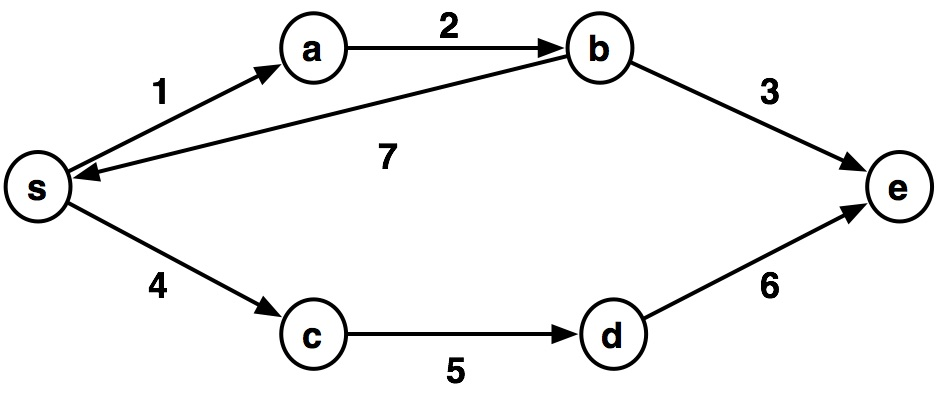
\includegraphics[width=3.0in]{shortest-paths/weighted-graph}
\end{center}
\label{ex:shortestpath::pathlength}
\end{example}

For a weighted graph $G(V,E,w)$ a shortest weighted path from vertex
$u$ to vertex $v$ is a path from $u$ to $v$ with minimal weight.
%
There might be multiple paths with equal weight; if so they are all
shortest weighted paths from $u$ to $v$.  
%
We use the term \defn{distance} from $u$ to $v$, written
$\delta_G(u,v)$, to refer to the weight of a shortest path from $u$ to
$v$.
%
If there is no path from $u$ to $v$, then we define the distance
to be infinity, i.e., $\delta_G(u,v) = \infty$.
%







\begin{question}
What is  the (weighted) shortest path from $s$ to $e$? 
\end{question}
\begin{answer}
In the graph above, the shortest path from $s$ to $e$ is $\langle
s,a,b,e \rangle$ with weight $6$.
\end{answer}


\begin{question}
What happens if we change the weight of the edge $(b,s)$ from $7$ to $-7$?
\end{question}

Recall that a path allows for repeated vertices----a simple path does
not.
%
If we allow for negative weight edges then it is possible to create
shortest paths of infinite length (in edges) and whose weight
is~$-\infty$.  
%
In \exref{shortestpath::pathlength} if we change the weight of the
edge $(b,s)$ to $-7$ the shortest path between $s$ and $e$ has weight
$-\infty$ since a path can keep going around the cycle
$\cseq{s,a,b,s}$ reducing its weight by $4$ each time around.
%
For this reason, when computing shortest paths we will need to be
careful about cycles of negative weight.  
%
As we will discover, even if there are no negative weight cycles,
negative edge weights make finding shortest paths more difficult.
%
For this reason, we will first consider the problem of finding
shortest paths when there are no negative edge weights.  
%


In this chapter, we are interested in finding single-source shortest
paths as defined in \probref{sp::sssp} below.
%
Note that the problem requires finding  only one of the possibly many
shortest paths between two vertices.  
%
In some cases, we only care about the distance $\delta(u,v)$ but not
the path itself.

\begin{problem}[Single-Source Shortest Paths (\sssp)]
\label{prob:sp::sssp}
  Given a weighted graph $G = (V,E,w)$ and a source vertex $s$, the
  \defn{single-source shortest path (\sssp) problem} is to find a
  shortest weighted path from $s$ to every other vertex in $V$.
\end{problem}


%We will refer to this variant of the \sssp{}
%problem as the \ssspd{} problem.


In \secref{gs::bfs} we saw how Breadth-First Search (BFS) can be used to
solve the single-source shortest path problem on graphs without edge
weights, or, equivalently, where all edges have weight $1$.
\begin{question}
Can we use BFS to solve the single-source shortest path problem on
weighted graphs?
\end{question}
Ignoring weight and using BFS, unfortunately, does not work on
weighted graphs.

\begin{example}
To see why BFS does not work, consider the following
directed graph with $3$ vertices:
%
\begin{center}
  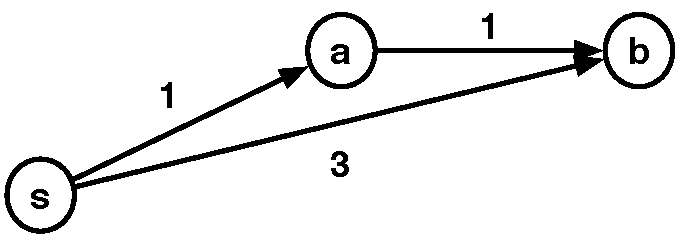
\includegraphics[width=2.0in]{shortest-paths/breaking-bfs-1}
\end{center}
%
BFS first visits $b$ and then $a$.  When it visits~$b$, it assigns $b$
an incorrect weight of~$3$. 
%
Since BFS never visit~$b$ again, it will not find the shortest path
going trough~$a$, which happens to be shorter.
\end{example}

\begin{examplenotes}
Another graph where BFS fails to find the shortest paths correctly
%
\begin{center}
  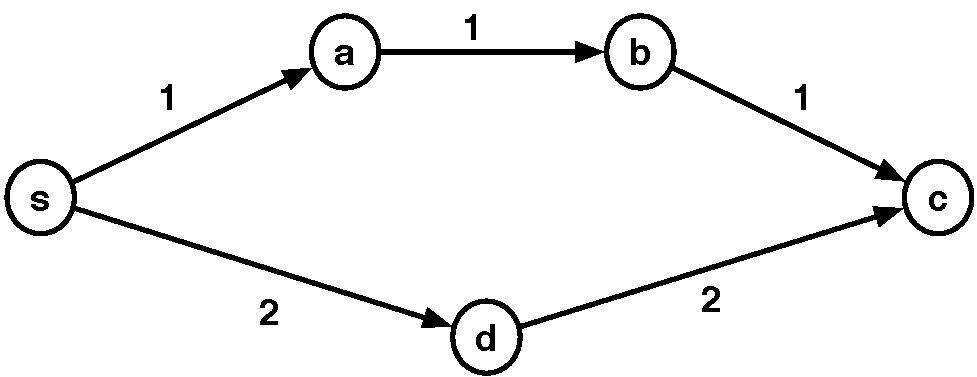
\includegraphics[width=3.0in]{shortest-paths/breaking-bfs-2}
\end{center}
%
\end{examplenotes}

\begin{comment}
\begin{question}
Can you see why BFS works on graphs without edge weights?
\end{question}
\end{comment}

The reason why BFS works on unweighted graphs is quite interesting and
helpful for understanding other shortest path algorithms.  The key
idea behind BFS is to visit vertices in order of their distance from
the source, visiting closest vertices first, and the next closest, and
so on.  More specifically, for each frontier $F_i$ (at round $i$), BFS
has the correct distance from the source to each vertex in the
frontier.  It then can determine the correct distance for
unencountered neighbors that are distance one further away (on the
next frontier).  We will use a similar idea for weighted paths.

\begin{comment}
\begin{remark}
One way to think of BFS, especially when reasoning about shortest
paths, is to think of a ``gadget'' where each vertex is a bucket and
each edge is a pipe that connects the buckets. Imagine now pumping
water into the ``source'' bucket and watch the gadget flooded with
water.  The way water floods the system simulates how BFS discovers
the paths and vertices.  The flood waters reach a vertex through the
shortest path first, because they discover all paths simultaneously
arriving at each place at the earliest possible time.
\end{remark}
\end{comment}



%% Let's consider using a similar approach when the graphs has
%% non-negative edge weights. Starting from the source vertex $s$, for which
%% vertex can we safely say we know its shortest path from $s$?  The
%% vertex $v$ that is the closest
%% neighbor of $s$.  There could not be a shorter path to $v$, since such
%% a path would have to go through one of the neighbors that is further
%% away from $s$ and that path cannot get shorter because none of the
%% edge weights are negative.  More generally, if
%% we know the shortest path distances for a set of vertices, how can we
%% determine the shortest path to another vertex?
%% This is the question that Dijkstra's algorithm answers.



\section{Dijkstra's Algorithm}

Consider a variant of the \sssp{} problem, where all the weights on
the edges are non-negative (i.e. $w : E \to \R^+)$.  We refer to this
as the \defn{\ssspp{} problem}. 
%
Dijkstra's algorithm solves the \ssspp{} problem.  It is an important
algorithm, because it is efficient, and because it is an elegant
example of a greedy algorithm that can find optimal results.
%
In this section, we are going to (re-)discover this algorithm by
taking advantage of properties of graphs and shortest paths.  

Let's start by noting that since no edges have negative weights, there
cannot be a negative-weight cycle.  
%
One can therefore never make a path shorter by visiting a vertex
twice---i.e., a path that cycles back to a vertex cannot have less
weight than the path that ends at the first visit to the vertex. 
%
When searching for a shortest path, we thus have to consider only the
simple paths.

\begin{question}
Give a brute-force algorithm for finding the shortest path?
\end{question}

Let us start with a brute-force algorithm for the \ssspp{} problem,
that, for each vertex, considers all simple paths between the source
and the vertex and selects the shortest such path.
%
\begin{question}
How many simple paths can there be between two vertices in a graph?
\end{question}
%
Unfortunately there can be a large number (exponential in the number
of vertices) of paths between any pair of vertices, so any algorithm that
tries to look at all paths is not likely to scale beyond very small
instances.
%
We therefore have to try to reduce the work. 
%
\begin{question}
Why does the brute-force algorithm does redundant work? 
\end{question}
%
Toward this end let us observe that the brute-force algorithm does
redundant work, because it does not take advantage of a crucial
property of shortest paths: any sub-path of a shortest path is a
shortest path (between its end vertices).
%
We refer to this property as the \defn{sub-paths property} of shortest
paths.
%
This property means that we can build shortest paths from smaller
shortest paths.
%
We are going to use this property to derive both Dijkstra's algorithm,
and also Bellman-Ford's algorithm, which solves the \sssp{} problem on
general graphs, allowing for negative edge weights.

\begin{example}[Subpaths property]
If a shortest path from Pittsburgh to San Francisco goes through
Chicago, then that shortest path includes the shortest path from
Pittsburgh to Chicago.   
\end{example}


To see how sub-paths property can be helpful, consider the graph in
\exref{shortestpath::allbutone} and suppose that an oracle has told us
the shortest paths to all vertices except for the vertex~$v$.  We want
to find the shortest path to~$v$.
%
\begin{question}
Can you find the shortest path to~$v$?
\end{question}
%
By inspecting the graph, we know that the shortest path to~$v$ goes
through either one of $a$, $b$, or $c$. Furthermore, by sub-paths
property, we know that the shortest path to~$v$ consists of the
shortest path to one of $a$, $b$, or~$c$, and the edge to~$v$.  Thus,
all we have to do is to find the vertex $u$~among the in-neighbors
of~$v$ that minimizes the distance to~$v$, i.e., $\dist_G(s,u)$ plus
the additional edge weight to get to~$v$.
%
\begin{question}
Could the shortest-path be going through~$v$?  If so, then are we
still guaranteed to find a shortest path?
\end{question}
%
Recall that we have decided to find only the shortest paths that are
simple, which cannot go through~$v$ itself.


\begin{example}
  In the graph $G$ shown below, suppose that we have found the
  shortest paths from the source~$s$ to all the other vertices except
  for~$v$; each vertex is labeled with its distance to $s$. The weight
  of the shortest path to~$v$ 
%
\\ 
%
is~$\min{
\left(
\dist_G(s,a) + 3,
%
\dist_G(s,b) + 6,
%
\dist_G(s,c)+5
\right)
}$.
%
The shortest path goes through the vertex
  ($a,b$, or $c$) that minimizes the weight, which in this case is
  vertex $b$. 

\begin{center}
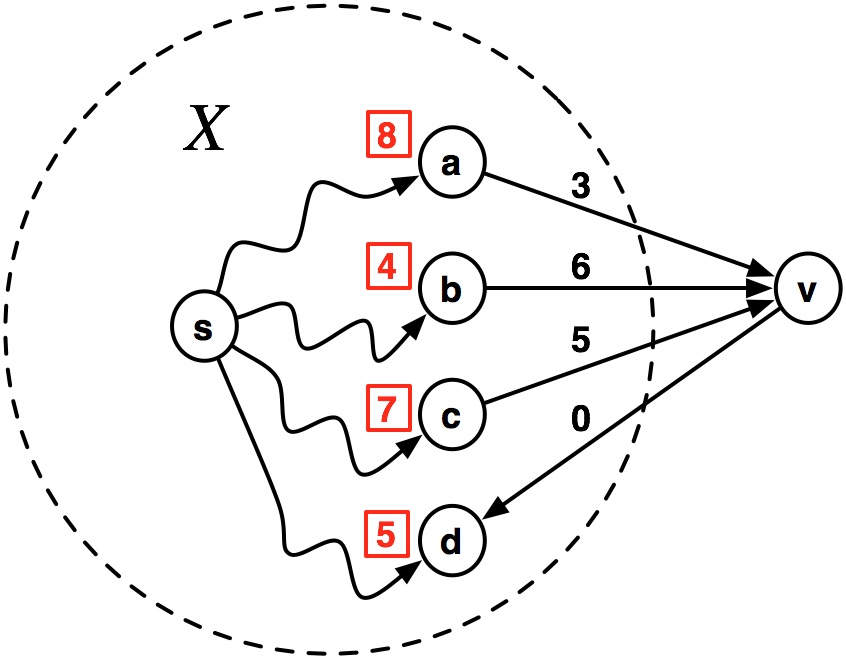
\includegraphics[width=3in]{shortest-paths/shortest-paths-last}
\end{center}
\label{ex:shortestpath::allbutone}
\end{example}


\begin{notesonly}
Let's now consider the case where the oracle gave us the shortest path
to all but two of the vertices~$u,v$. 
\begin{question}
 Can we find the shortest path to any one of $u$ or $v$?
\end{question}

Let~$X$ denote the set of vertices for which we know the shortest
paths.
%
Let's calculate for $u$ (and $v$) the shortest path that goes through
a neighbor in~$X$ and then goes to $u$ ($v$). Consider now the
shortest of these two distances and assume without loss of generality
that it is the path to~$u$.  Assume that the path is strictly smaller.

\begin{question}
Could the shortest path to~$u$ be this path? 
\end{question}

Since source is in $X$, we know that the shortest paths to~$u$ cross
out from~$X$ via some edge that goes to either~$u$ or~$v$. Since we
know that the weight of such a path to~$u$ is the smaller, and since
all edge weights are non-negative, there cannot be a shorter path that
goes to~$v$ and than comes back to~$u$ again.  
%
If the path is not strictly smaller, again the path that goes out to
$v$ and comes back to $u$ is going to be no shorter.
%
We thus conclude that the shortest path to~$u$ is the path that we
have found by considering all incoming edges
from~$X$. \exref{shortestpath::allbuttwo} illustrates this.


\begin{example}
\label{ex:shortestpath::allbuttwo}
In the following graph, suppose that we have found the shortest paths
from the source $s$ to all the vertices in $X$.  The shortest paths
are indicated by labels next to the vertices.  
%
The shortest path from the source $s$ to vertex $u$ in $Y$ is the
path to vertex $d$ with weight $5$ followed by the edge $(d,u)$ with
weight $4$ and hence total weight $9$.  
%
If edge weights are non-negative there cannot be any shorter way to
get to $u$, whatever $w(v,u)$ is, therefore we know that $\delta(s,u)
= 9$.
\begin{center}
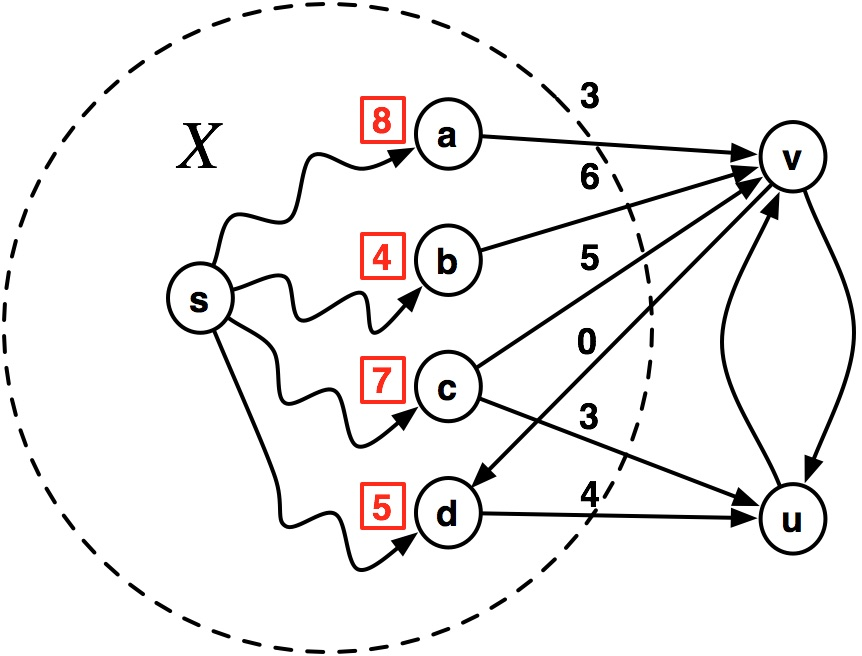
\includegraphics[width=3in]{shortest-paths/shortest-paths-all-but-two}
\end{center}

\end{example}

\begin{question}
Can you see how we can generalize this idea?  
\end{question}

\end{notesonly}


Let's try to generalize the argument and consider the case where the
oracle tells us the shortest paths from $s$ to to some subset of the
vertices $X \subset V$ with $s \in X$.  
%
Also let's define $Y$ to be the vertices not in $X$, i.e. $V\setminus
X$.  
%
Consider this question: can we  efficiently determine the shortest path
to any one of the vertices in~$Y$.
\begin{question}
What would be the point of doing that? 
\end{question}
If we could do this, then we would have an algorithm to add new
vertices to $X$ repeatedly, until we are done.  As in graph search, we
call the set of vertices that are neighbors of $X$ but not in $X$,
i.e. $N^+(X) \setminus X$, the frontier.

It should be clear that any path that leaves $X$ has to go through a
frontier vertex on the way out.  Therefore for every $v \in Y$ the
shortest path from $s$ must start in $X$, since $s \in X$, and then
leave $X$ via a vertex in the frontier.
\begin{question}
Can you use this property to identify a vertex $v \in Y$ that is no
farther from the source than any other vertex in $Y$?
\end{question}
Consider the vertex $v \in Y$ that has an edge to some already visited
vertex $x \in X$ and that minimizes the sum $\dist_G(s,x) + w(x,v)$.
Since all paths to $Y$ must go through the frontier when exiting $X$,
and since edges are non-negative, a sub-path cannot be longer than the
full path.  Thus, no other vertex in $Y$ can be closer to the source
than $x$. See \exref{shortestpath::some}. Furthermore, since all other
vertices in $Y$ are farther than $v$ and since all edges are
non-negative, the shortest path for $v$ is $\dist_G(s,x) + w(x,v)$.


\begin{example}
  In the following graph suppose that we have found the shortest paths
  from the source $s$ to all the vertices in $X$ (marked by numbers
  next to the vertices).  The shortest path from the source $s$ to a
  vertex $u$ in $Y$ is the path to vertex $d$ with weight $5$ followed by
  the edge $(d,u)$ with weight $4$ and hence total weight $9$.  If
  edge weights are non-negative there cannot be any shorter way to get
  to $u$, whatever $w(v,u)$ is, therefore we know that $\delta(s,u) =
  9$.
\begin{center}
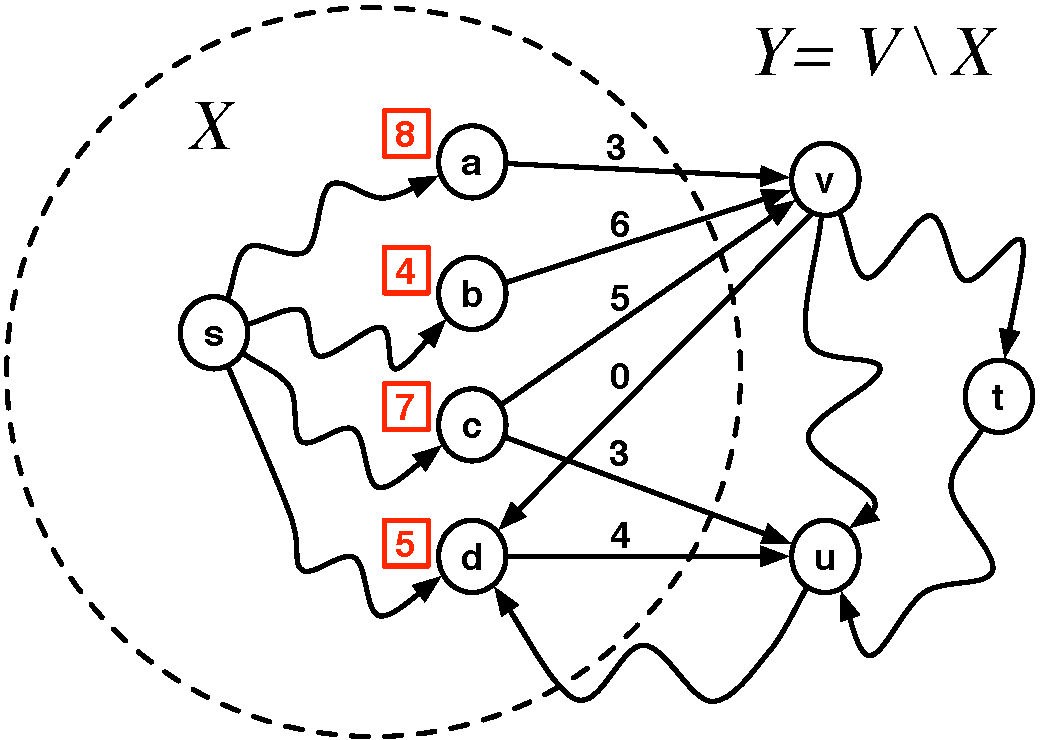
\includegraphics[width=3in]{shortest-paths/shortest-paths-some}
\end{center}
\label{ex:shortestpath::some}
\end{example}


\begin{figure}
\begin{lemma}[Dijkstra's Property] \label{lem:sp::djk}
  Consider a (directed) weighted graph $G = (V,E, w)$, $w\!: E \to \R^*$, and a source vertex $s \in V$.  
Consider any partitioning of the vertices $V$ into $\visited$ and
$Y = V \setminus \visited$ with $s \in \visited$,  and let
\[p(v) \equiv \min_{x \in X} (\dist_G(s,x) + w(x,v))\]
then $\displaystyle \min_{y \in Y} p(y) = \min_{y \in Y} \dist_G(s, y)$.
\vspace{-.2in}
\begin{center}
  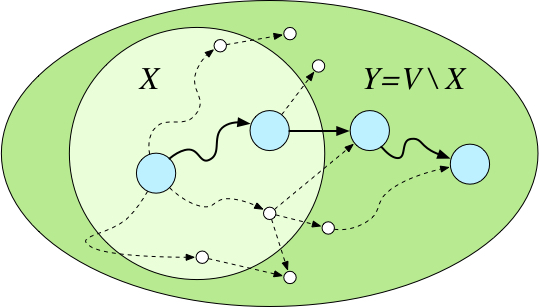
\includegraphics[width=3in]{shortest-paths/dijkstra-prop}
\end{center}

In English: \defn{The overall shortest-path weight from $s$ via a
  vertex in $X$ directly to a neighbor in $Y$ (in the frontier) is as
  short as any path from $s$ to any vertex in $Y$.}
\begin{proof}
  Consider a vertex $v_m \in Y$ such that $\dist_G(s,v_m) = \min_{v
    \in Y} \dist_G(s, v)$, and a shortest path from $s$ to $v_m$ in
  $G$.  The path must go through an edge from a vertex $v_x \in X$ to
  a vertex $v_t$ in $Y$ (see the figure).  Since there are no negative
  weight edges, and the path to $v_t$ is a sub-path of the path to
  $v_m$, $\dist_G(s,v_t)$ cannot be any greater than $\dist_G(s,v_m)$
  so it must be equal.  We therefore have $ \min_{y \in Y} p(y) \leq \dist_G(s,v_t) = \dist_G(s,v_m) =\min_{y \in Y} \dist_G(s, y)$, but the leftmost term cannot
  be less than the rightmost, so they must be equal.
\begin{comment}
  The path must cross from $X$ to $Y$ at some point using some
  edge $(v_X,v_T)$. Since sub-paths of shortest paths are shortest
  paths, the sub-path from $s$ to $v_T$ is a shortest path to $v_T$
  and, since edges are non-negative, path weights do not decrease along
  the path implying $\dist_G(s,v_T) \leq \dist_G(s,v_m)$ (it could
  be that $v_T = v_m$).  Furthermore $\min_{x \in X} (\dist_G(s,x) +
  w(x,v_T)) = \dist_G(s,v_T)$ by assumption, which gives the desired
  result since:
\[
d_{XY} \leq \min_{x \in X} (\dist_G(s,x) + w(x,v_t)) = \dist_G(s,v_t) \leq \dist_G(s,v_m)
= \min_{y \in Y} \dist_G(s, y)\, .\]
and
\[d_{XY} \geq \min_{y \in Y} \dist_G(s, y)\, ,\]
since $d_{XY}$ are path weights to $Y$ and the right hand side is the
overall shortest path to $Y$, so together we have an equality.
\end{comment}
\end{proof}
Implication: \emph{ This gives us a way to easily find $\dist_G(s,v)$
  for at least one vertex $v \in Y$.  In particular for all $v \in Y$
  where $p(v) = \min_{y \in Y} p(y)$, it must be the case that $p(v) =
  \dist_G(s,v)$ since there cannot be a shorter path.  Also we need
  only consider the frontier vertices in calculating $p(v)$,
  since for others in $Y$, $p(y)$ is infinite.  }
\end{lemma}
\end{figure}

The intuition that we have developed thus far is stated more precisely
and proved in \lemref{sp::djk}.  
%
The Lemma tells us that once we know
the shortest paths to a set $X$ we can add more vertices to $X$ with
their shortest paths.  This gives us a crank that can churn out at
least one new vertex on each round. Dijkstra's algorithm simply does
exactly this: it turns the crank until all vertices are visited.


You might have noticed that the terminology that we used in explaining
Dijkstra's algorithm closely relates to that of graph search.
%
\begin{question}
  Does this algorithm remind you of a particular graph search that we
  discussed?
\end{question}
%
More specifically, recall that priority search is a graph search,
where each round visits the frontier vertices with the highest
priority.  
%
If as usual we denote the visited set by~$X$, we can define the
priority for a vertex~$v$ in the frontier,~$p(v)$, as the weight of
the shortest-path weight consisting of a path to~$x \in X$ and an
additional edge from~$x$ to~$v$.  In other words, this algorithm is
actually an instance of priority-first search.
%
We are now ready to define precisely Dijkstra's algorithm.
\begin{algorithm}[Dijkstra's Algorithm]
  For a weighted graph $G=(V,E,w)$ and a source $s$, Dijkstra's
  algorithm is priority search on $G$ starting at $s$ with $d(s) = 0$,
  using priority $\displaystyle p(v) = \min_{x \in X} (d(x) + w(x,v))$
  (to be minimized), and setting $d(v) = p(v)$ when $v$ is visited.
\end{algorithm}
%
Note that Dijkstra's algorithm will visit vertices in non-decreasing
shortest-path weight since on each round it visits unvisited vertices
that have the minimum shortest-path weight from~$s$.


\begin{comment}
\begin{figure}
\begin{pseudocode}
~\\
\begin{lstlisting}
function $\sssppd(G, s) =$ 
let
   $D = \cset{s \mapsto 0}$     
   $F = N(s)$        % the frontier
  while $|F| \neq 0$ with $(D,F)$     % $D$ is a table from $v \in X$ to $\dist_G(s,v)$ 
     $\displaystyle D_F = \cset{y \mapsto \min_{(x \mapsto d) \in D}(d + w(x,y)) : y \in F}$
     $\displaystyle d_{XY} = \min_{(y \mapsto d) \in D_F} d$
     $Y = \csetf{(y \mapsto d) \in D_F}{d = d_{XY}}$
     $D = D \cup Y$
     $F = (F \cup N_G(Y)) \setminus \mbox{domain}(D)$
in
  $X$
end
\end{lstlisting}
\label{alg:pfsdjk}
\end{pseudocode}
\end{figure}
\end{comment}



\begin{remark}
It may be tempting to think that Dijkstra's algorithm visits vertices
strictly in increasing order of shortest-path weight from the source,
visiting vertices with equal shortest-path weight on the same round.
This is not true. To see this consider the example below and convince
yourself that it does not contradict our reasoning.

\begin{center}
  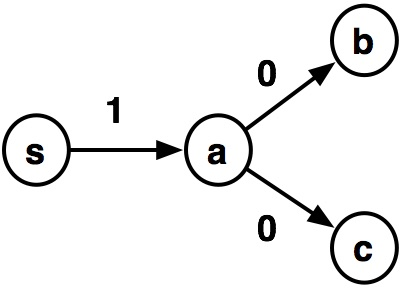
\includegraphics[width=1.5in]{shortest-paths/dijkstra-zero-weight-counter-example}
\end{center}
\end{remark}

\begin{lemma}
  Dijkstra's algorithm returns~$d(v) = \delta_G(s,v)$ for~$v$ 
  reachable from~$s$.
\begin{proof}
  We show that for each step in the algorithm, for all $x \in X$ (the
  visited set), $d(x) = \delta_G(s,x)$.  This is true at the start
  since $X = \cset{s}$ and $d(s) = 0$.  On each step the search adds
  vertices $v$ that minimizes $P(v) = \min_{x \in X} (d(x) + w(x,v))$.
  By our assumption we have that $d(x) = \delta_G(s,x)$ for $x \in X$.
  By \lemref{sp::djk}, $p(v) = \delta_G(s,v)$, giving $d(v) =
  \delta_G(s,v)$ for the newly added vertices, maintaining the
  invariant.  As with all priority-first searches, it will eventually
  visit all reachable $v$.
\end{proof}
\end{lemma}


\subsection{Implementation and the Cost of Dijkstra's Algorithm}

We can implement Dijkstra's algorithm efficiently using a priority
queue to maintain $p(v)$ as shown in \algref{sp::dijkstra}.
%
The algorithm uses a priority queue that supports \cname{deleteMin}
and \cname{insert} operations. 
%
Note that this algorithm only adds one vertex at a time even if
there are multiple vertices with equal distance.


%%% Commenting out these invariants.
%%% These might be helpful for implementation.

\begin{figure}[tb]
\begin{algorithm}[Dijkstra's Algorithm using Priority Queues]~
\begin{lstlisting}[numbers=left]
dijkstraPQ ($G$,$s$) = 
let
  requires:
     $\forall {(x \mapsto d) \in X}, d = \dist_G(s,x)$     
     $
     \begin{array}{ll}
      \csetf{(d,y) \in Q}{y \in V \setminus X} = 
          \{ (d + w(x,y), y): & (x \mapsto d) \in X,
      \\
      & y \in N_G^+(x) \setminus X 
           \}
     \end{array}
     $
  returns: $\cset{x \mapsto \dist_G(s,x) : x \in R_G(s)} $
  function dijkstra ($X$, $Q$) = 
    case @\fbox{PQ.deleteMin}@($Q$) of  @\label{line:dijkstra::min}@        
     ($\cnone$, _) => $X$
    | $(\csome{(d,v)}, Q')$ =>  
        if @\fbox{$(v,\_) \in X$}@ then  @\label{line:dijkstra::find}@        
          dijkstra ($X$, $Q'$)
        else
          let  @\label{line:dijkstra::let}@ 
           $X'$ = @\fbox{$X \cup \{(v,d)\}$}@ @\label{line:dijkstra::insert}@
           relax ($Q$, ($u$, $w$)) = @\fbox{PQ.insert}@($d+w$, $u$) $Q$ @\label{line:dijkstra::pqinsert}@   
           $Q''$ = @\fbox{iterate}@ relax $Q'$ @\fbox{$N_G^+(v)$}@ @\label{line:dijkstra::iter}@
          in dijkstra ($X'$, $Q''$) end      
in
  dijkstra ($\{\}$, @\fbox{PQ.insert}@($0$, $s$) $\{\}$)   @\label{line:dijkstra::end}@
end
\end{lstlisting}
\label{alg:sp::dijkstra}
\end{algorithm}
\end{figure}

The algorithm maintains the visited set $\visited$ as a table mapping
each visited vertex $u$ to $d(u) = \delta_G(s,u)$.  It also maintains
a priority queue $Q$ that keeps the frontier prioritized based on the
shortest distance from $s$ directly from vertices in $\visited$.  On each
round, the algorithm selects the vertex $x$ with least distance $d$ in
the priority queue (\lineref{dijkstra::min} in the code) and, if it
hasn't already been visited, visits it by adding $(x \mapsto d)$ to
the table of visited vertices (\lineref{dijkstra::insert}), and then
adds all its neighbors $v$ to $Q$ along with the priority $d(x) +
w(x,v)$ (i.e. the distance to $v$ through $x$)
(\linereftwo{dijkstra::pqinsert}{dijkstra::iter}).  
%
Note that a
neighbor might already be in $Q$ since it could have been added by
another of its in-neighbors.  $Q$ can therefore contain duplicate
entries for a vertex, but what is important is that the minimum
distance will always be pulled out first.  \lineref{dijkstra::find}
checks to see whether a vertex pulled from the priority queue has
already been visited and discards it if it has.  This algorithm is just
a concrete implementation of the previously described Dijkstra's
algorithm.

\begin{comment}
\begin{remark}
As with the BFS algorithm, we can think of Dijkstra's algorithm as
flooding the graph from the source. The only difference is that we
have to think of the weights as the time for the water to traverse a
pipe (edge).  
\end{remark}
\end{comment}

\begin{figure}
\begin{example}
An example run of Dijkstra's algorithm. Note that after
visiting~$s$,~$a$, and~$b$, the queue~$Q$ contains two distances
for~$c$ corresponding to the two paths from~$s$ to~$c$ discovered thus
far.  The algorithm takes the shortest distance and adds it to~$X$.  A
similar situation arises when $c$ is visited, but this time
for~$d$. Note that when~$c$ is visited, an additional distance for~$a$
is added to the priority queue even though it is already visited.
Redundant entries for both are removed next before visiting~$d$.  The
vertex~$e$ is never visited as it is unreachable from~$s$.  Finally,
notice that the distances in~$X$ never decrease.


\begin{center}
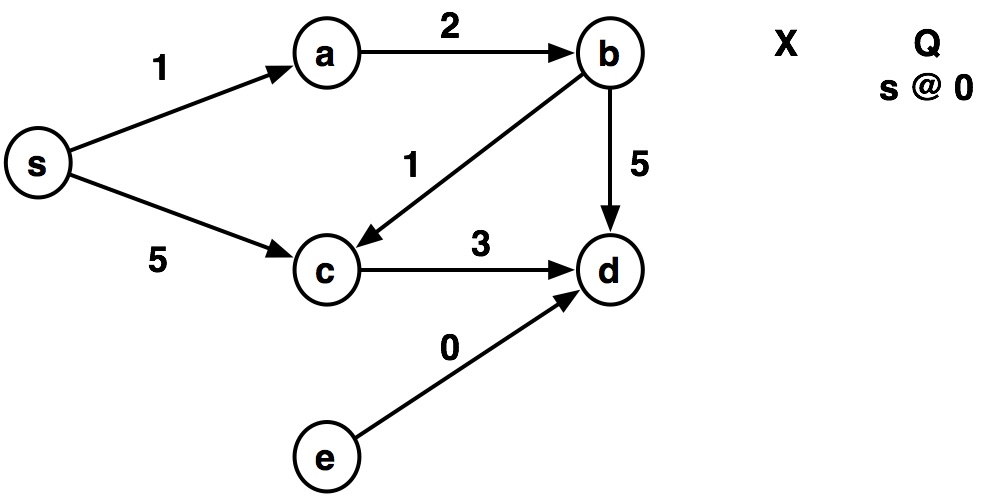
\includegraphics[width=2.75in]{shortest-paths/dijkstra-0} 
\hfill
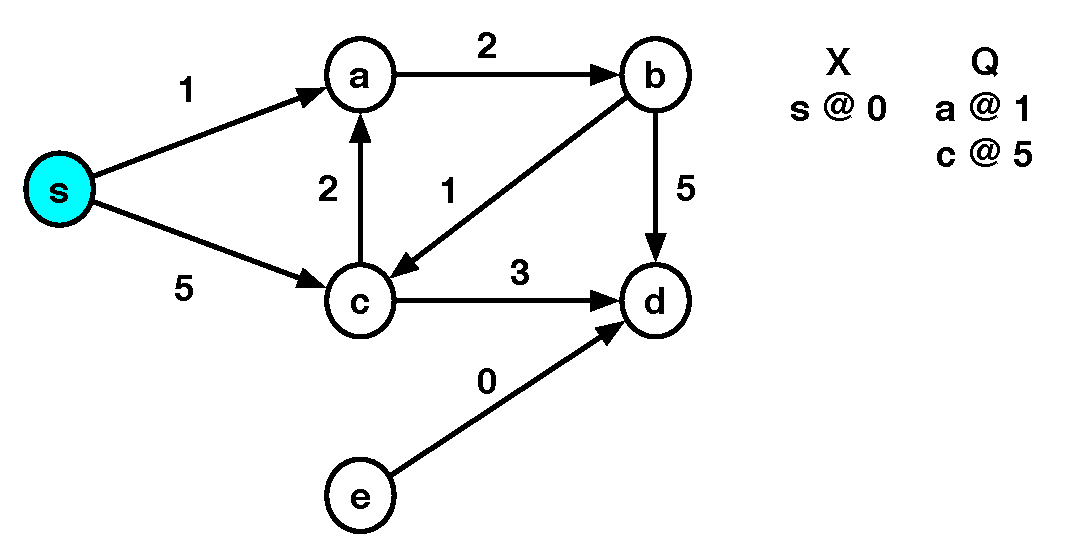
\includegraphics[width=2.75in]{shortest-paths/dijkstra-1}
\vspace{5ex}
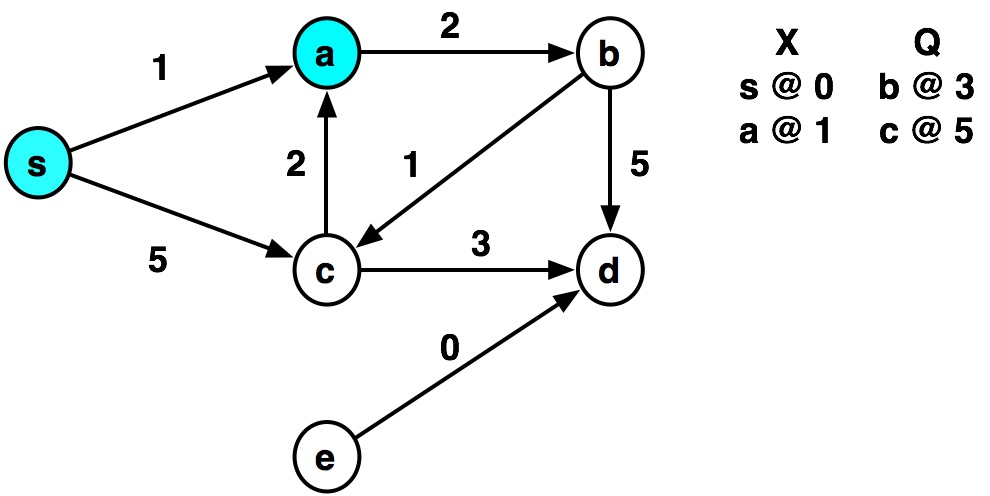
\includegraphics[width=2.75in]{shortest-paths/dijkstra-2}
\hfill
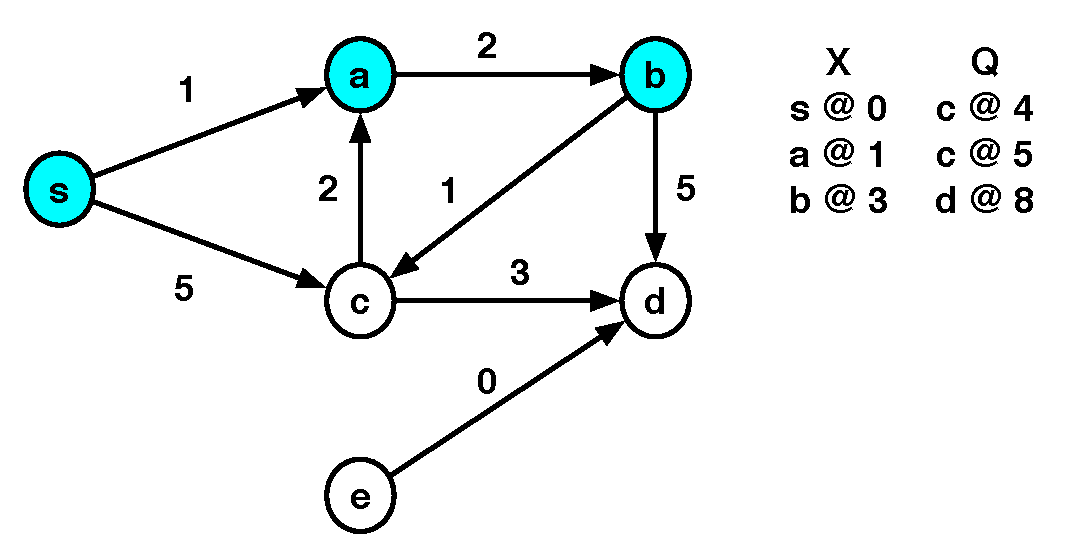
\includegraphics[width=2.75in]{shortest-paths/dijkstra-3}
\vspace{5ex}
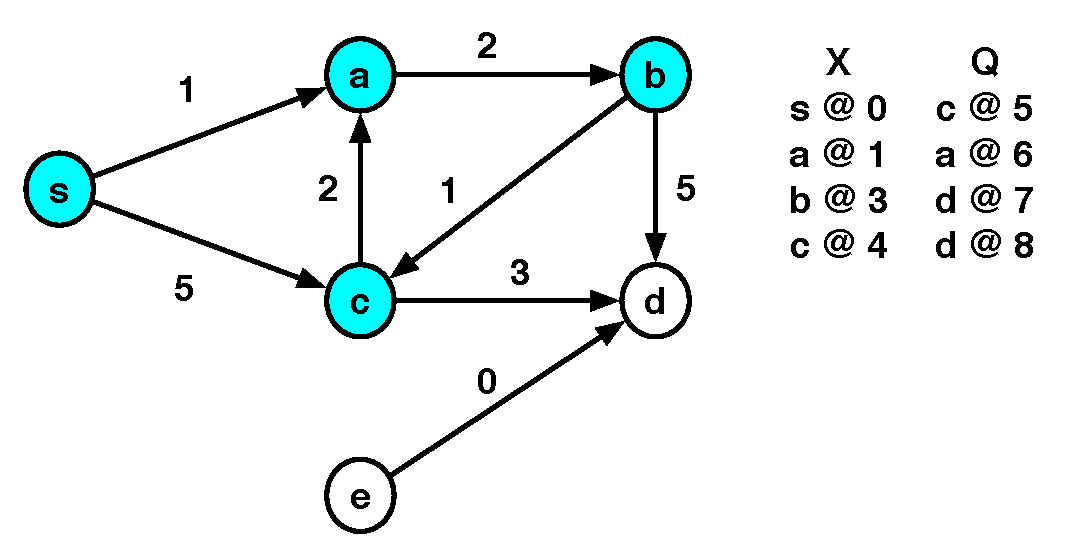
\includegraphics[width=2.75in]{shortest-paths/dijkstra-4}
\hfill 
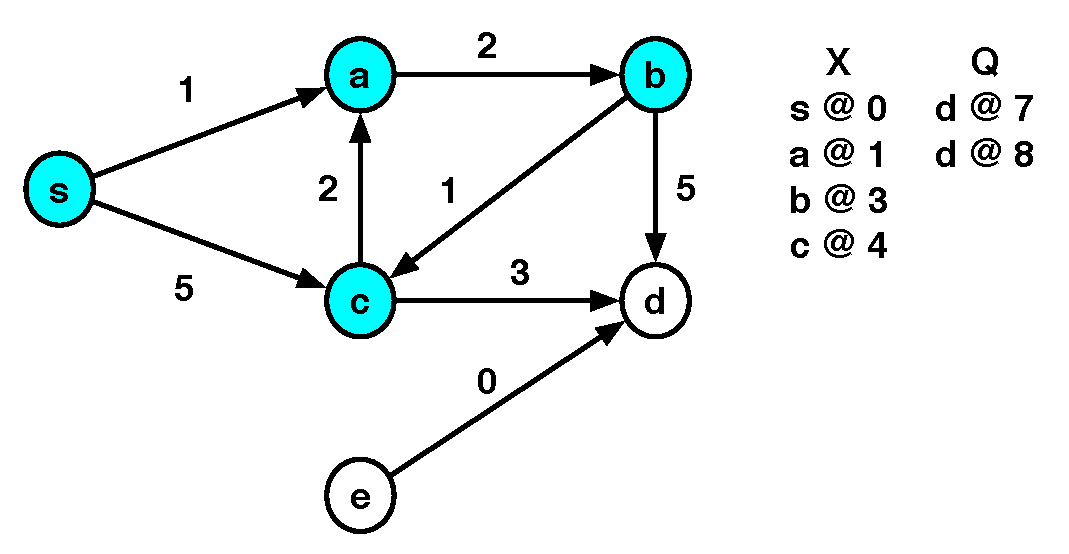
\includegraphics[width=2.75in]{shortest-paths/dijkstra-5}
\vspace{5ex}
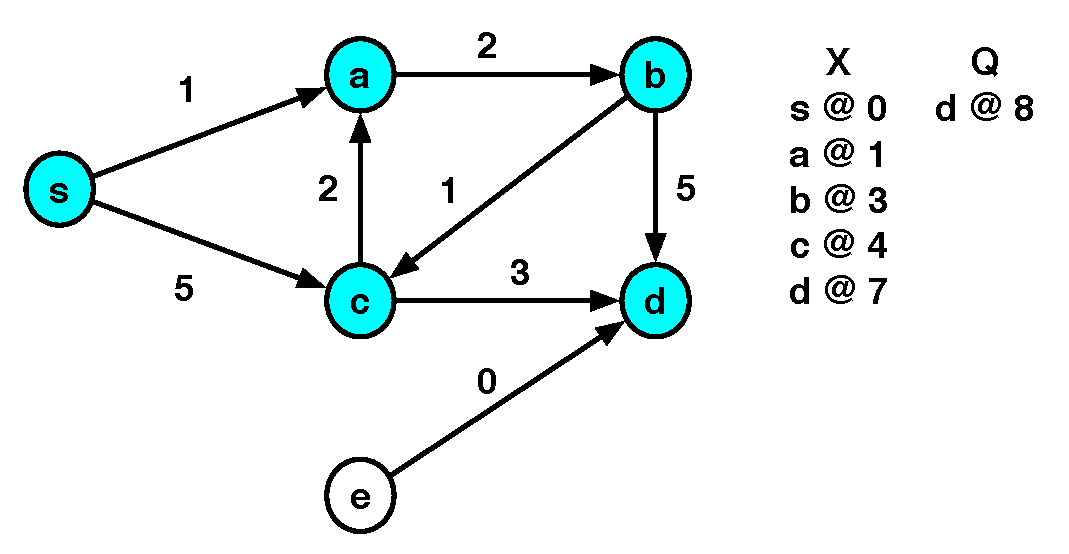
\includegraphics[width=2.75in]{shortest-paths/dijkstra-6}
\hfill
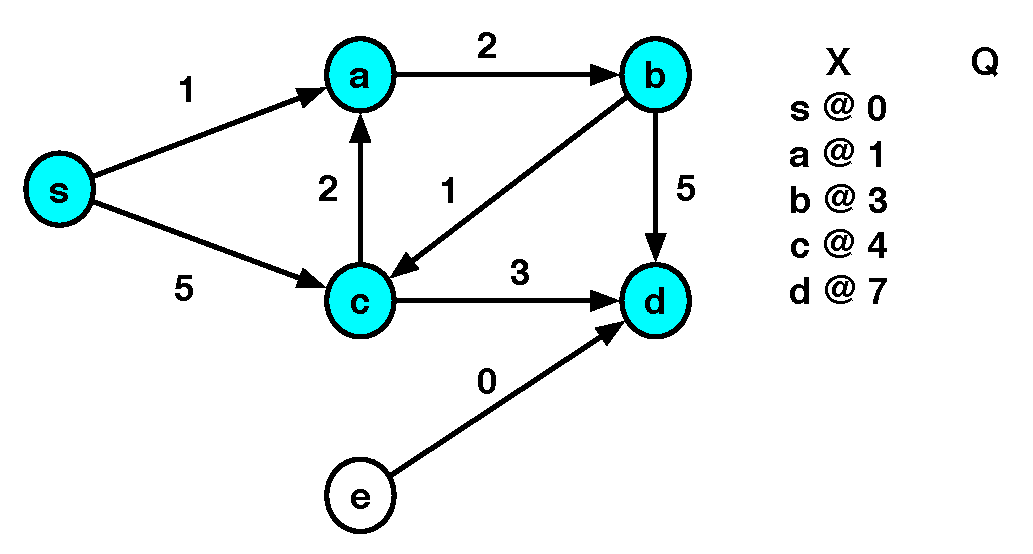
\includegraphics[width=2.75in]{shortest-paths/dijkstra-7}
\end{center}
\end{example}
\end{figure}

There are a couple other variants on Dijkstra's algorithm using
priority queues. 
%
Firstly we could check inside the \cname{relax} function whether $u$
is already in $X$ and if so not insert it into the priority queue.
%
This does not affect the asymptotic work bounds but probably would
give some improvement in practice.  
%
Another variant is to decrease the priority of the neighbors instead
of adding duplicates to the priority queue.  This requires a more
powerful priority queue that supports a \cname{decreaseKey} function.


To analyze the work and span of priority-queue based implementation of
Dijkstra's algorithm shown in \algref{sp::dijkstra}, let's first
consider the priority queue ADT's that we use.
%
For the priority queue, we assume \cname{PQ.insert} and
\cname{PQ.deleteMin} have $O(\log n)$ work and span.  
%
Since Dijkstra's algorithm makes no updates to the graph, we can
represent the input graph simply either by using a table or a
sequence, mapping vertices to their out-neighbors along with the
weight of the corresponding edge.
%
As we shall see, it suffices to use the tree based costs for tables.
%
To represent the mapping of visited vertices to their distances, we
can use a table, an array sequence, or a single-threaded array
sequences.
%

To analyze the work, we calculate the work for each different kind of
operation and sum them up to find the total work.
\figref{sp::dijkstra-costs} summarizes the costs of the operations,
along with the number of calls made to each operation.

The algorithm includes a box around each operation on the graph $G$,
the set of visited vertices $X$, or the priority queue $\cname{PQ}$.
The \cname{PQ.insert} in \lineref{dijkstra::end} is called only once,
so we can safely ignore it.  Of the remaining operations, The
\cd{iterate} and $N_G^+(v)$ on \lineref{dijkstra::iter} are on the
graph, \linereftwo{dijkstra::find}{dijkstra::insert} are on the table
of visited vertices $X$, and
\linereftwo{dijkstra::min}{dijkstra::pqinsert} are on the priority
queue $Q$.


\begin{figure}
%\begin{tabular}{llc|c|c|c|c|c} 
\begin{tabular}{llcccccc} 
\toprule
%
& Operation & Line & \# of calls & PQ & Tree Table & Array & ST Array
\\ 
%
\midrule
%
&\cname{deleteMin} &\lineref{dijkstra::min}
& $O(m)$      & $O(\log m)$ & - & - & - \\
&\cname{insert} & \lineref{dijkstra::pqinsert}
& $O(m)$ & $O(\log m)$ & - & - & -\\ 
\midrule
%%
% \multicolumn{3}{l|}{\bf Priority Q total}
% &        & $O(m \log m)$ & - & - & -
% \\
% \hline
%%
& \cname{find} & \lineref{dijkstra::find}
& $O(m)$     & -           & $O(\log n)$ & $O(1)$ & $O(1)$ \\
& \cname{insert} & \lineref{dijkstra::insert}
& $O(n)$   & -           & $O(\log n)$ & $O(n)$ & $O(1)$ \\ 
\midrule
%%
% \multicolumn{3}{l|}{\bf Distances total}
% &        & -             & $O(m \log n)$ & $O(n^2)$ & $O(m)$ \\ 
%\hline
%%
& $N_G^+(v)$ & \lineref{dijkstra::iter}
& $O(n)$      & -           & $O(\log n)$ & $O(1)$ & - \\
& \cd{iterate} & \lineref{dijkstra::iter}
& $O(m)$     & -           & $O(1)$ & $O(1)$ & - \\ 
%%
%\hline
%\multicolumn{3}{l|}{\bf Graph access total}
%&        & -             & $O(m + n \log n)$ & $O(m)$ & -\\ 
%%
\bottomrule
%\bf Total & - & $O(m \log n)$ & $O(m \log n)$ & $O(n^2)$ & $O(m)$ \\ \hline
\end{tabular}
\caption{The costs for the important steps in the algorithm \cname{dijkstraPQ}.}
\label{fig:sp::dijkstra-costs}
\end{figure}

We can calculate the total number of calls to each operation by noting
that the body of the let starting on \lineref{dijkstra::let} is only
run once for each vertex.  Thus, \lineref{dijkstra::insert} and
$N_G^+(v)$ on \lineref{dijkstra::iter} are only called $O(n)$ times.
All other operations are performed once for each edge.  The total work
for Dijkstra's algorithm using a tree table is therefore $O(m \log m +
m \log n + m + n \log n)$.  Since $m \le n^2$, the total work is $O(m
\log n)$.

Since the algorithm is sequential, the span is the same as the work.

Based on the table one should note that when using either tree tables
or single threaded sequences, the cost is no more than the cost of the
priority queue operations.  Therefore there is no asymptotic advantage
of using one over the other; there might, however, be differences in
constant factors.  One should also note that using regular purely
functional arrays is not a good idea, because the cost is then
dominated by the insertions and the algorithm runs in $\Theta(n^2)$
work.





\section{The Bellman Ford Algorithm}

We now turn to solving the single source shortest path problem in the
general case where we allow negative weights in the graph.  One might
ask how negative weights make sense.  When considering distances on a
map for example, negative weights do not make sense (at least without
time travel), but many other problems reduce to shortest paths. In
such reductions negative weights do show up.

Before proceeding we note that if there is a negative weight cycle
(the sum of weights on the cycle is negative) reachable from the
source, then there cannot be a finite-distance solution to the
single-source shortest path problem, as discussed earlier.
%
In such a case, we would like the algorithm to indicate that such a
cycle exists and terminate.

\begin{notesonly}
\begin{todo}
 In the graph above, one student has found a cycle that allows
dollar to be converted more dollars.  You might want to update the example. 

These rates from Oct 26, 2016.

\end{todo}

\begin{exercise}
  Consider the following \defn{currency exchange} problem: given a set
  currencies, a set of exchange rates between them, and a source
  currency $s$, find for each other currency $v$ the best sequence of
  exchanges to get from $s$ to $v$.  Hint: how can you convert
  multiplication to addition.

Here is an example:

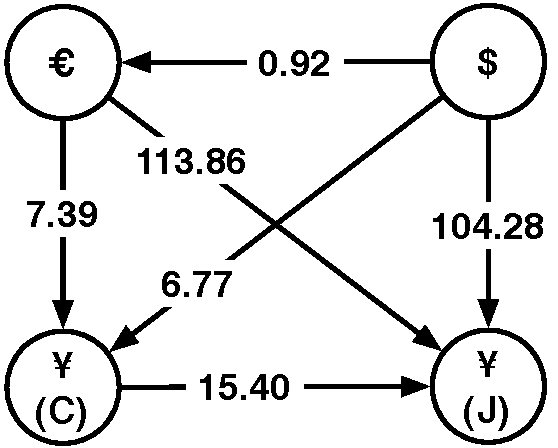
\includegraphics[width=3in]{shortest-paths/currency-exchange}

In the general case, you can imagine having $n$ currencies and finding
the best way to convert a currency into another.


\end{exercise}




We can convert multiplication to addition by taking logs.  But we also
need to convert longest, which is what we want, to shortest.  So we
have to use negative log. 


\begin{exercise}
In your solution to the previous exercise can you get negative weight
cycles?   If so, what does this mean?
\end{exercise}

\end{notesonly}

\begin{question}
Why can't we use Dijkstra's algorithm to compute shortest path when
there are negative edges?
\end{question}

Recall that in our development of Dijkstra's algorithm we assumed
non-negative edge weights.  This both allowed us to only consider
simple paths (with no cycles) but more importantly played a critical
role in arguing the correctness of Dijkstra's property.  More
specifically, Dijkstra's algorithm is based on the assumption that the
shortest path to the vertex $v$ in the frontier that is closest to the
set of visited vertices, whose distances have been determined, can be
determined by considering just the incoming edges of $v$.  With
negative edge weights, this is not true anymore, because there can be a
shorter path that ventures out of the frontier and then comes back to
$v$.


\begin{example}
To see where Dijkstra's property fails with negative edge weights
consider the following example.
\begin{center}
  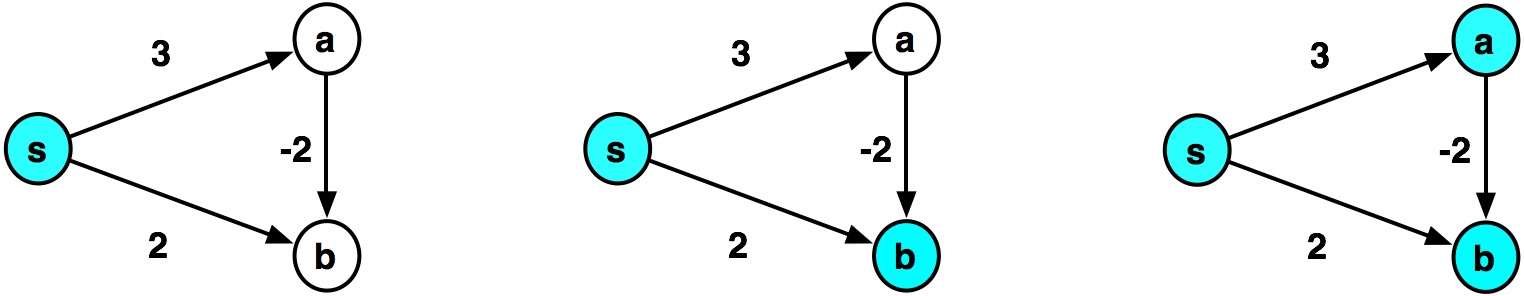
\includegraphics[width=5in]{shortest-paths/dijkstra-negative}
\end{center}
Dijkstra's algorithm would visit $b$ then $a$ and leave $b$ with a
distance of $2$ instead of the correct distance $1$.  The problem is
that when Dijkstra visits $b$, it fails to consider the possibility of
there being a shorter path from $a$ to $b$ (which is impossible with
non-negative edge weights).
\end{example}

\begin{question}
How can we find shortest paths on a graph with negative weights?
\end{question}
\begin{question}
Recall that for Dijkstra's algorithm, we started with the brute-force
algorithm and realized a key property of shortest paths.  Do you
recall the property?
\end{question}

A property we can still take advantage of, however, is that the
sub-paths of a shortest paths themselves are shortest. 
%
Dijkstra's algorithm exploits this property by building longer paths
from shorter ones, i.e., by building shortest paths in non-decreasing
order.  
%
With negative edge weights this does not work anymore, because
paths can get shorter as we add edges.

\begin{question}
Is there another way to use this property?
\end{question}

But there is another way to use the same property: building paths that
contain more and more edges.  To see how, suppose that you have found
the shortest paths from source to all vertices with~$k$ or fewer
edges.
%
\begin{question}
  How can you update the shortest paths for $k+1$ edges? That is you
  want to find the shortest paths that contain $k+1$ or fewer edges.
\end{question}
%
We can compute the shortest paths with $k+1$ or fewer edges by
extending all paths by one edge if this is beneficial. 
%
To find the shortest paths with at most $k+1$ edges, all we need to do
is consider each vertex $v$ and all its incoming edges and pick the
shortest path to that vertex that arrives at a neighbor $u$ using $k$
or fewer edges and then takes the edge $(u,v)$.
%
To make this more precise, define \defn{k-distance}, written
$\delta^k_G(s,t)$, as distance from $s$ to $t$ considering all paths
with at most $k$ edges, i.e., the shortest weighted path from $s$ to
$t$ using at most $k$ edges.
%


\begin{example}
  In the following graph $G$, suppose that we have found the shortest
  paths from the source $s$ to vertices using $k$ or fewer edges; each
  vertex $u$ is labeled with its $k$-distance to $s$, written
  $\dist_G^k(s,u)$. The weight of the
  shortest path to~$v$ using $k+1$ or fewer edges is 
%
\[
\min
\left(
\dist_G^k(s,v),\min{\dist_G^k(s,a)+3, \dist_G^k(s,b)-6,\dist_G^k(s,c)+5}
\right
.
\]
%
The shortest path with at most $k+1$ edges has weight $-2$ and goes
through vertex $b$.

\begin{center}
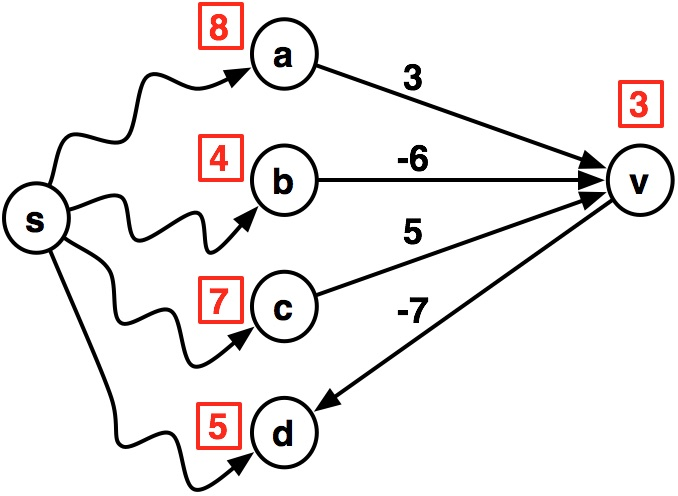
\includegraphics[width=2.5in]{shortest-paths/shortest-paths-last-negative}
\end{center}
\label{ex:shortestpath::allbutone-negative}
\end{example}

Based on this idea, we can construct paths with greater number of
edges.  We start by determining $\delta^0_G(s,v)$ for all $v \in V$.
5
Since no vertex other than the source is reachable with a path of
length $0$, $\delta^0_G(s,v) = \infty$ for all vertices other than the
source.  
%
Then we determine $\delta^1_G(s,v)$ for all $v \in V$, and
iteratively, $\delta^{k+1}_G(s,v)$ based on all $\delta^{k}_G(s,v)$
for all $k > 1$.
%
To calculate the updated distances with at most $k+1$ edges the
algorithm, we can use the shortest path with $k$ edges to each of its
in-neighbors and then adds in the weight of the one additional edge.
More precisely, for each vertex $v$,
\[
\delta^{k+1}(v) = \min(\delta^{k}(v),\min_{x \in N^-(v)}
(\delta^{k}(x) + w(x,v))\;).
\]
Recall that $N^-(v)$ indicates the in-neighbors of vertex $v$.

\begin{question}
Can the distances for a vertex stays the same? 
\end{question}
Since the new distance for a vertex is calculated in terms of the
distances from most recent iteration, if the distances for all
vertices remain unchanged, then they will continue remaining unchanged
after one more iteration.  
%
\begin{question}
When should we stop? 
\end{question}
%
It is therefore unnecessary to continue iterating after the distances
converge---we can stop when distances converge.
%
\begin{question}
Is convergence guaranteed?  
\end{question}
Convergence, however is not guaranteed.  For example, if we have a
negative cycle reachable from the source then, some distances
continue to decrease at each iteration.
%
\begin{question}
Can we detect such a situation? 
\end{question}
%
We can detect negative cycles by noticing that the distances do not
converge even after $|V|$ iterations.  This is because, a simple
(acyclic) path in a graph can include at most $|V|$ edges and, in the
absence of negative-weight cycles, there always exist an acyclic
shortest path.



\begin{figure}[tb]
\begin{algorithm}[Bellman Ford]~
\begin{lstlisting}
BellmanFord $(G=(V,E),s)$ = 
let
   requires: $\forall {v \in V}, D_v = \delta_G^k(s,v)$
   BF $(D,k)$ =
   let
      $D' = \{v \mapsto \min(D[v],\min_{u \in N_G^-(v)} (D[u] + w(u,v))) : v \in V \}$ @\label{line:bf::distances}@
   in 
     if $(k = |V|)$ then $\cnone$ @\label{line:bf::negcycle}@
     else if (all$\cset{D[v] = D'[v] : v \in V}$) then $\csome{D}$ @\label{line:bf::if}@
     else $BF(D',~k+1)$
   end 

   $D = \cset{v \mapsto~\infty : v \in V \setminus \{s\}} \cup 
        \cset{s \mapsto 0}$

in $BF(D,0)$ end
\end{lstlisting}
\label{alg:sp::bf-code}
\end{algorithm}
\end{figure}

\algref{sp::bf-code} defines the Bellman Ford algorithm based on these ideas.
%It assumes we have added a zero weight self loop on the
%source vertex.  
%
The algorithm runs until convergence or until $|V|$ iterations have
been performed.
%
If $|V$ iterations have been performed and the distances did not
converge, then in \lineref{bf::negcycle}, the algorithm returns
\cnone.
%
This indicates that the algorithm has detected a negative weight
cycle.
%
An illustration of the
algorithm over several steps is shown in \exref{sp::bf}.
\begin{figure}
\begin{example}
\label{ex:sp::bf}

Several steps of the Bellman Ford algorithm.  The numbers with squares
indicate the current distances and highlight those that has changed on
each step.


\begin{center}
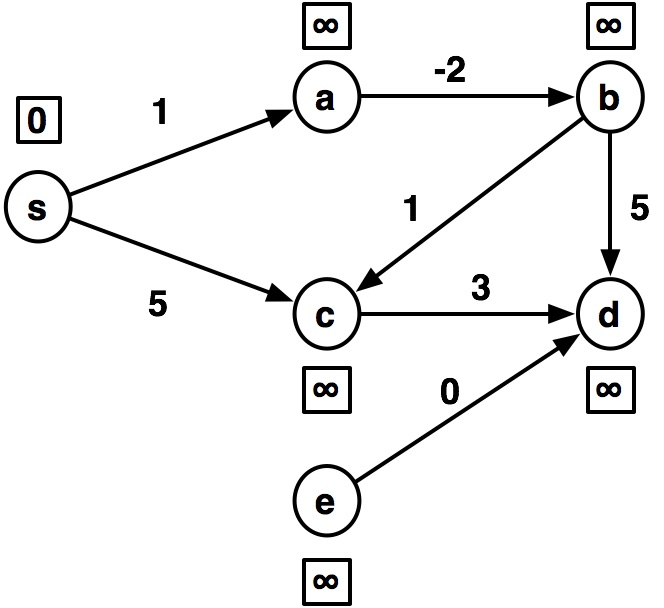
\includegraphics[width=2.0in]{shortest-paths/bf-0} 
\hspace{1in}
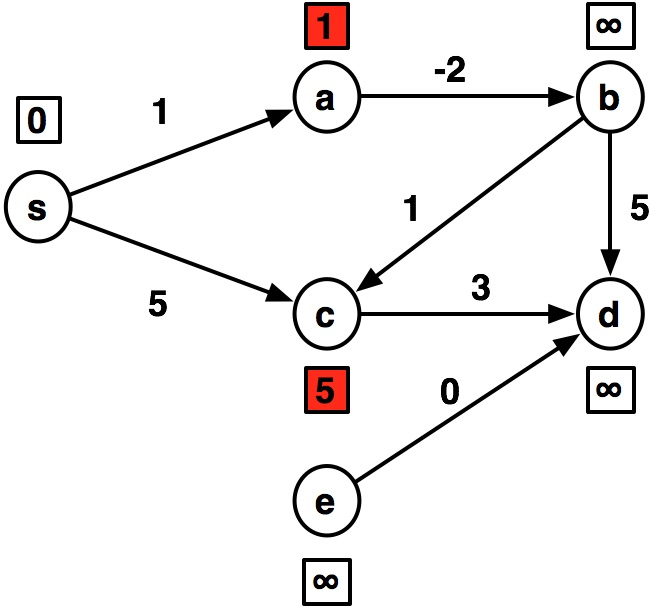
\includegraphics[width=2.0in]{shortest-paths/bf-1}
\\[10ex]
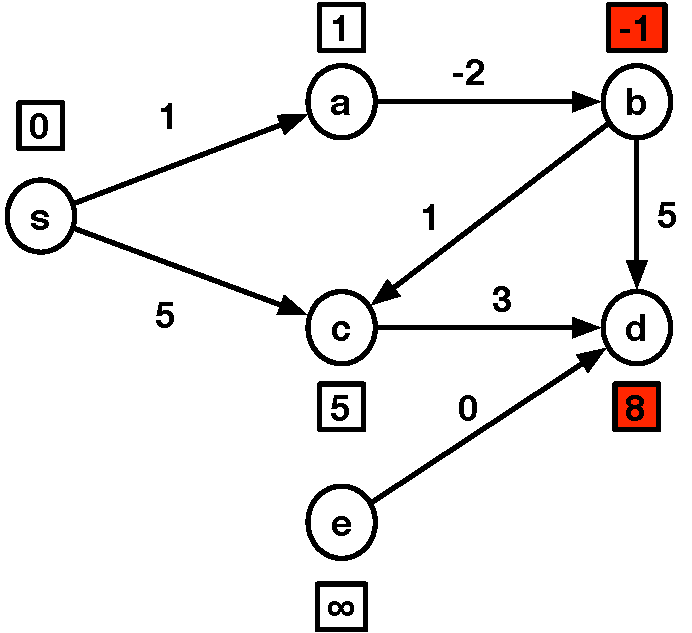
\includegraphics[width=2.0in]{shortest-paths/bf-2}
\hspace{1in}
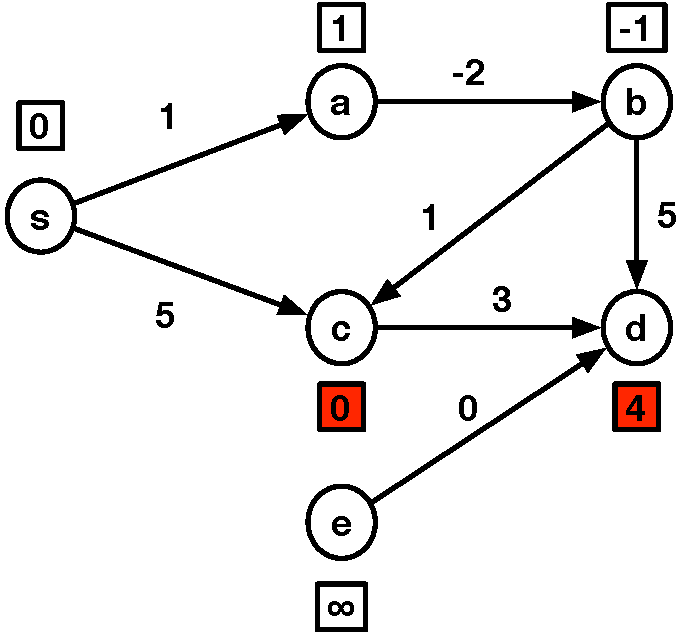
\includegraphics[width=2.0in]{shortest-paths/bf-3}
\\[10ex]
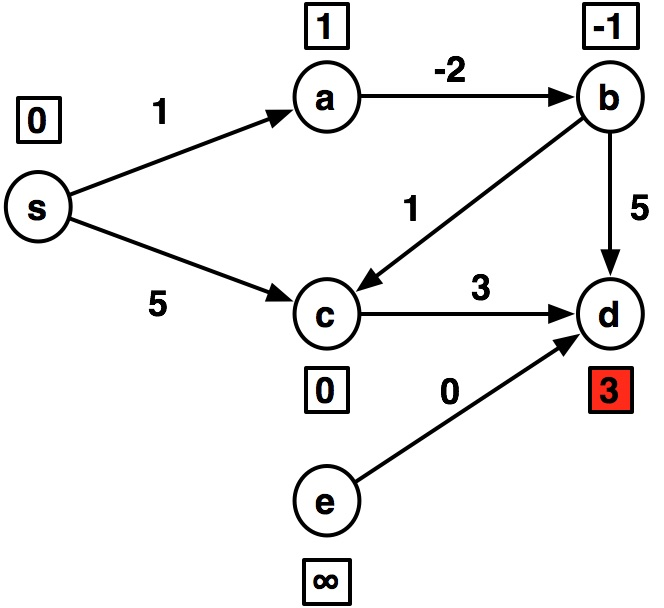
\includegraphics[width=2.0in]{shortest-paths/bf-4}
\end{center}

\end{example}
\end{figure}


\begin{theorem}
  Given a directed weighted graph $G = (V,E,w)$, $w : E \to R$, and a
  source $s$, the \cname{BellmanFord} algorithm returns either
  $\dist_G(s,v)$ for all vertices reachable from $s$, or indicates
  that there is a negative weight-cycle in $G$ that is reachable from
  $s$.
\end{theorem}
\begin{proof}
  By induction on the number of edges $k$ in a path.  The base case is
  correct since $D_s = 0$.  For all $v \in V\setminus{s}$, on each
  step a shortest $(s,v)$ path with up to $k+1$ edges must consist of
  a shortest $(s,u)$ path of up to $k$ edges followed by a single edge
  $(u,v)$.  Therefore if we take the minimum of these we get the
  overall shortest path with up to $k+1$ edges.  For the source the
  self edge will maintain $D_s = 0$.    The algorithm can only proceed
  to $n$ rounds if there is a reachable negative-weight cycle.   
  Otherwise a shortest path to every $v$ is simple and can consist of
  at most $n$ vertices and hence $n-1$ edges.
\end{proof}  

\subsection{Cost of Bellman-Ford}

For the cost analysis cost of Bellman-Ford, we consider two different
representations for graphs, one using tables and the other using
sequences.
%
For a table-based representation of the graph, we use a table mapping
each vertex to a table of neighbors along with their real-valued
weights.
%
We represent the distances $D$ as a table mapping vertices to their
distances.
%

Let's consider the cost of one call to $BF$, not including the
recursive calls.  The only nontrivial computations are on
\linereftwo{bf::distances}{bf::if}. \lineref{bf::distances} consists of a
tabulate over the vertices. 
%
As the cost specification for tables indicate, to calculate the work
for a tabulate, we take the sum of the work for each vertex, and for
the span we take the maximum of the spans, and add $O(\log n)$.  
%
Now consider what the algorithm does for each vertex.  First, it has
to find the neighbors in the graph (using a \texttt{find G v}).  This
requires $O(\log |V|)$ work and span. 
%
Then the algorithm performs a map over the  in-neighbors. 
%
Each instance of this map requires finding in the distance table to
obtain $D[u]$, finding in the weight table, the weight, and an
addition operation.  
%
The find operations take $O(\log |V|)$ work and span.  
%
Finally there is a reduce for finding the shortest path through an
in-neighbor.  The reduce takes $O(1 + |N_G(v)|)$ work and $O(\log
|N_G(v)|)$ span.  
%
For each vertex the value calculated by mapping over the neighbors is
compared against the current distance $D[v]$ and the minimum is
taken.  This requires $O(\lg |V|)$ work and span.
%
Using $n = |V|$ and $m = |E|$, we can write the work
as follows
\begin{eqnarray*}
W_{BF}(n,m)
& = & O\left(\sum_{v \in V} \left(\log n + |N_G^-(v)| + \sum_{u
  \in N_G^-(v)} (1 + \log n)\right)\right) 
\\
& = & O\left((n + m) \log n\right). 
\end{eqnarray*}
%
The first term is for looking up the current distance, the second term
is for reduce, and the third term is the cost for mapping over the
neighbors.


Similarly,  we can write the span as follows
\begin{eqnarray*}
S_{BF}(n,m)
& = & O\left(\max_{v \in V} \left(\log n + \log |N_G^-(v)| + \max_{u
  \in N_G^-(v)} (1 + \log n)\right)\right) 
\\
& = & O(\log n). 
\end{eqnarray*}
%
The work and span of \lineref{bf::if} is simpler to analyze since it only
involves a tabulate and a reduction: it requires $O(n \log n)$ work
and $O(\log n)$ span.

Since the number of calls to $BF$ is bounded by $n$, as discussed
earlier.  Since the calls to \cd{BF} are performed sequentially, we
can multiply the work and span for each call by the number of calls to
compute the total work and span, which, assuming $m \ge n$, are
\begin{eqnarray*}
W_{BF}(n,m) & = & O(n m \log n)\\
S_{BF}(n,m) & = & O(n \log n).\\
\end{eqnarray*}

Let's now analyze the cost with a sequence representation of graphs.
%
If we assume that the graphs is unemerable, then the vertices are
identified by the integers $\{0,1,\ldots,|V|-1\}$ and we can use
sequences to represent the graph. 
%
Instead of using a \cd{find} for a table, which requires $O(\log
n)$ work, we can use \cd{nth} (indexing) requiring only $O(1)$
work.  
%
This improvement in costs can be applied for looking up in the
graph to find the neighbors of a vertex, and looking up in the
distance table to find the current distance.  By using the improved
costs we get:
\begin{eqnarray*}
W_{BF}(n,m) & = & O\left(\sum_{v \in V} \left(1 + |N_G^-(v)| + \sum_{u \in N_G^-(v)} 1\right)\right) \\
  & = & O(n+m) \\
S_{BF}(n,m) & = & O\left(\max_{v \in V} \left(1 + \log |N_G^-(v)| + \max_{u \in N_G^-(v)} 1\right)\right) \\
  & = & O(\log n) \\
\end{eqnarray*}
and hence the overall complexity for \cname{BellmanFord} with array
sequences is and assuming $m \ge n$,
\begin{eqnarray*}
W(n,m) & = & O(n m)\\
S(n,m) & = & O(n \log n)\\
\end{eqnarray*}
By using array sequences we have reduced
the work by a $O(\log n)$ factor.



%% \section{SML code}

%% Here we present the SML code for Dijkstra.


%% \begin{small}
%% \verbatiminput{../code/dijkstra.sml}
%% \end{small}

\begin{comment}
With this assumption, we seem close to an algorithm.  We have already
found a way to compute the shortest path to a vertex by using the
sub-paths property.  We can now iterate this process by taking out
vertices one by one and finding their shortest paths. Or inversely, we
can compute the shortest paths to some subset of the vertices and then
extend the set by adding another vertex.

\begin{question}
Would this algorithm work? 
\end{question}

This algorithm could work but only with a lot of luck.  To see why we
need a lot of luck, consider the example of the shortest path from
Pittsburgh to San Francisco and suppose that it goes through Chicago.
If in our algorithm, we consider San Francisco before Chicago, we will
not be able to find the shortest path to San Francisco.  Thus we now
have to solve the problem of how to order the vertices so that we can
find all shortest paths correctly.


\begin{question}
Can you pick an ordering on vertices so that all the shortest paths
would be computed correctly by this algorithm?
\end{question}

To solve this problem, suppose that we know the distance---that is the
weight of the shortest path---of each vertex to our source.  One idea
would be to visit the vertices in the order of their distances to the
source.  Let's see if this would work.  Suppose that we have found the
distance for all vertices up to distance~$d$ and we are now
considering a vertex~$v$ at distance~$d$; an example is shown below.

\begin{example}
\label{ex:dijkstra::monotone}

Finding the shortest path to a vertex~$v$ at distance~$d$ after
visiting all the vertices that are closer.  We can find a shortest
path to~$v$ by computing
$\min
\left(
\dist_G(s,a)+1,\dist_G(s,b)+\dist_G(s,c)+3
\right)
$.

\begin{center}
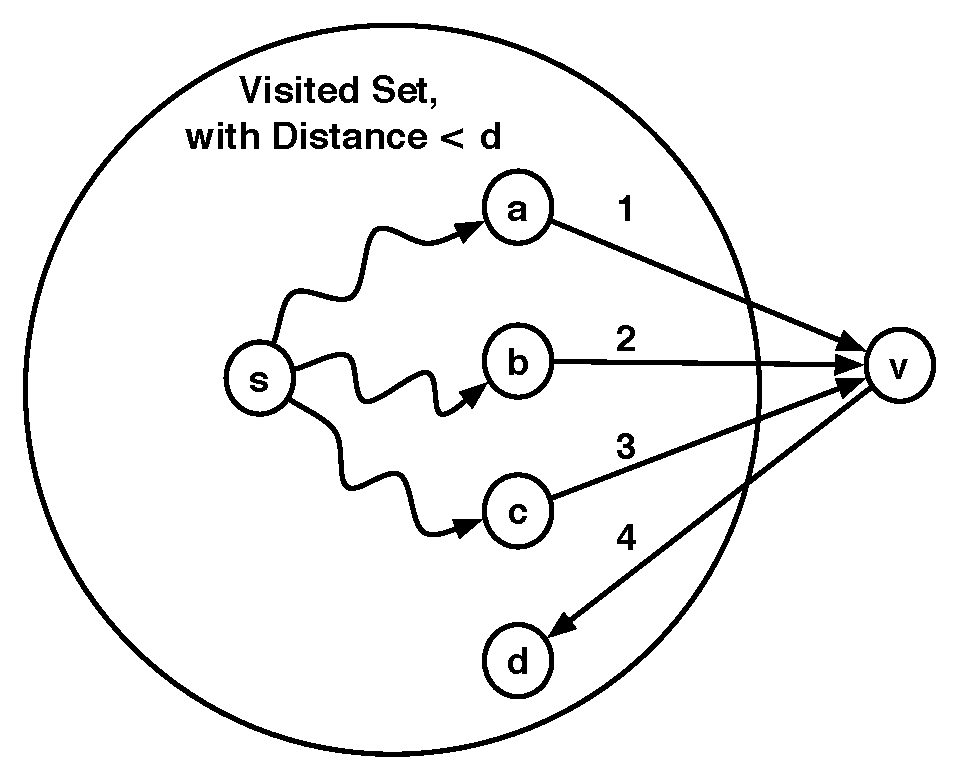
\includegraphics[width=3in]{shortest-paths/shortest-paths-distance-order}
\end{center}
\end{example}

\begin{question}
How can we find the shortest path to $v$?
\end{question}

Consider a shortest path to~$v$ and let $(u,v)$ be the last edge on
the path.  By sub-paths property, the shortest path to $u$ contains
the shortest path from source to~$u$.  Since all edges have positive
weights, $u$~is at a distance less than~$d$.  We therefore know
that~$u$ has been visited.  Thus to find the shortest path to~$v$, all
we have to do is to consider all incoming edges of~$v$ from the
visited set and compute the shortest path by taking the minimum of the
possibilities as shown in the example above.


The last piece of the puzzle remaining is to find the distance of the
vertices to the source, which we need in order to determine the
ordering for the shortest paths.  But this is a circular problem, how
can we find the ordering without finding the shortest paths?

\begin{question}
Can you think of a way of figuring out the order?
\end{question}

The key observation to solving this problem is to notice that we don't
have to know the order for all the vertices, we just have to know the
``next'' closest vertex to visit (at any point in the algorithm).

We are now going to show that having visited all the vertices at
distance less than~$d$, if we always pick the vertex closest to the
visited set, then we would be visiting vertices in increasing order of
distance from the source and we would find a shortest path to a vertex
when we visit that vertex.


\begin{example}
The distance of~$v$ to the visited set~$X$, denoted $\dist_{G,X}$ is
computed as $\dist_{G,X} = \min \left(\dist_G(s,a)+1, \dist_G(s,b)+2,
\dist_G(s,c)+3, \dist_G(s,d)+4 \right)$.  If~$v$ is the vertex in the
frontier with smallest such distance, then the distance of~$v$ to the
source is the smallest of all the remaining vertices. 

\begin{center}
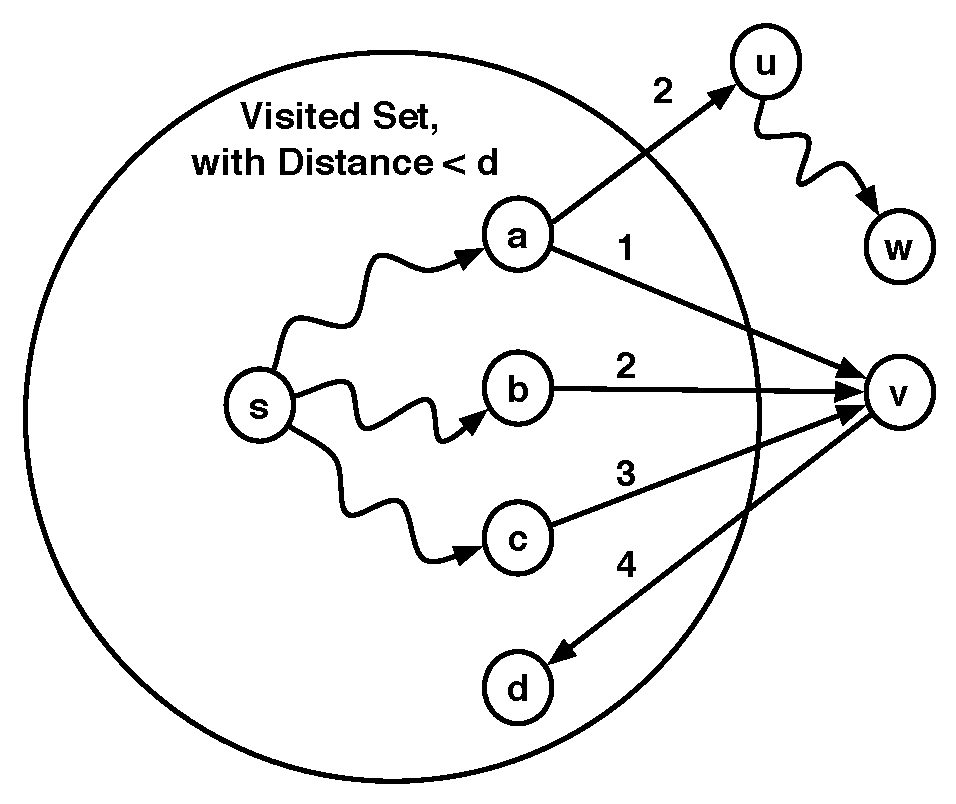
\includegraphics[width=3in]{shortest-paths/shortest-paths-distance-order-multi}
\end{center}
\end{example}

To prove this crucial property, let~$v$ be the vertex closest to the
visited set.  Assume for contradiction that there is another vertex~$w$,
not yet visited, whose distance is no less than $d$ but that is closer
to the source.  Consider a shortest path to~$w$ from the source and
let~$u$ be the first vertex outside~$X$.  Such a vertex exists because
each sub-path of the shortest path to~$w$ being considered is a
shortest path, and we have visited all the vertices with distance less
than~$d$. Since all edge weights are positive, the distance of~$u$ to
the visited set is smaller than that of~$v$.  But this is a
contradiction because we have picked~$v$ to be the vertex closest to
the visited set.  Thus, we conclude that no such~$w$ exists.

We have thus established that by picking~$v$, we have remained
consistent with the ordering of the vertices according to their
distance to the source.  


\begin{question}
Would we compute~$v$'s distance correctly?
\end{question}

This might seem like a redundancy but let's convince ourselves that we
can compute the distance of~$v$ to the source.  Thus far, we have only
computed the distance of~$v$ to the visited set. Since we have visited
all the vertices at distance less than~$d$ and since~$v$ is the
closest next vertex, we know that the computed path is a shortest path
from~$v$ to source, by our reasoning with increasing distances as in
\exref{dijkstra::monotone}.  In summary, what we have shown is that
the distance of~$v$ to the visited set is equal to its shortest path
distance to the source.


\begin{question}
Note that there can be many vertices with the same distance to the
visited set.  Does it matter which vertex is visited next.
\end{question}

Thus far, we have glossed over one detail: there can be multiple
vertices that have the same distance to the visited set.  It does not
matter, which one of these we pick because, all we need is that all
the vertices with shorter distances have been visited. We can thus
visit them in arbitrary order or in fact all in parallel.



\begin{question}
Can you generalize this reasoning to include zero-weight edges?
\end{question}

Thus far, we have assumed that all edges have positive weights.  This
is not a necessary assumption but greatly simplifies the reasoning
that we went through.  Dijkstra's algorithm actually satisfies an much
more elegant and simple property that can proved succinctly without
this assumption.  To truly understand this algorithm and appreciate
its beauty, you should make sure understand this property.

The key property used by Dijkstra's algorithm is that for a set of
vertices $X \subset V$ that include $s$ and the rest of the vertices
($\unvisited = V \setminus \visited$), the closest vertex in $T$ from
$s$ based on paths that only go through $X$ is also an overall
closest vertex in $T$.  This property will allow us to select the next
closest vertex by only considering the vertices we have already visited.
Defining $\dist_{G,X}(s,v)$ as the shortest
path length from $s$ to $v$ in $G$ that only goes through vertices in
$X$ (except for $v$), the property can be stated more formally and
proved as follows:

This lemma implies that if we have already visited a set of vertices
$\visited$ we can find a new shortest path to a vertex in $T = V
\setminus X$ by just considering the path lengths through $\visited$
to a neighbor of $\visited$.  In particular we want to pick a vertex
$t$ that minimizes $\delta_{G,X}(s,t)$.  This suggests an algorithm
for shortest paths based on priority first search using the priority
$P(v) = \delta_{G,\visited}(s,u)$.  Also note that
$\delta_{G,\visited}(u) = \min_{v \in V} (\delta_G(v) + w(v,t))$.
Indeed this gives us Dijkstra's algorithm, at
least in the abstract:

\begin{question}
Can you turn these ideas to an algorithm for computing the shortest
distances from a source to all the other vertices?
\end{question}

Based on these ideas, we can solve the single-source shortest paths
problem by maintaining a visited set of vertices whose distances have
already been computed correctly.  We then consider the vertices in the
frontier and calculate their distance by considering their incoming
edges.  We then extend the frontier by visiting the vertex with the
smallest computed vertex.  As usual we start our visited set with
source at distance zero.

This is in fact Dijkstra's algorithm.  
\end{comment}

\section{Problems}

\begin{probl}{}
There are 18 subgraphs for a triangle consisting of three vertices
and three edges connecting them, including the empty graph and the graph
itself.    List them all.
\end{probl}


\begin{probl}{}
In star contraction, what is the probability that a vertex with degree
$d$ is removed.
\end{probl}


\begin{probl}{}
Find an example graph, where star-based graph contraction removes a
small number of edges on each round.
\end{probl}

% Solution: a graph consisting of small stars that are connected with
% many edges. The star will be removed but all the cross edges between
% them will remain.  Must repeat this recursively to find the right
% structure.

\begin{probl}{}
Describe how to construct a graph that exhibits the worst-case
behavior for \thmref{gc::star-contraction-cost}.
\end{probl}

\begin{probl}{}
Is the star contraction algorithm work-optimal for a dense graph with
$\Omega(n^2)$ edges? Prove or disprove.
\end{probl}


\flushchapter
